\documentclass[tikz,border=8pt]{standalone}
\usepackage{amsmath,amssymb}
\usepackage{mathrsfs}
\usetikzlibrary{arrows.meta,calc,decorations.markings,decorations.pathmorphing,patterns,shapes.geometric,positioning}

\begin{document}
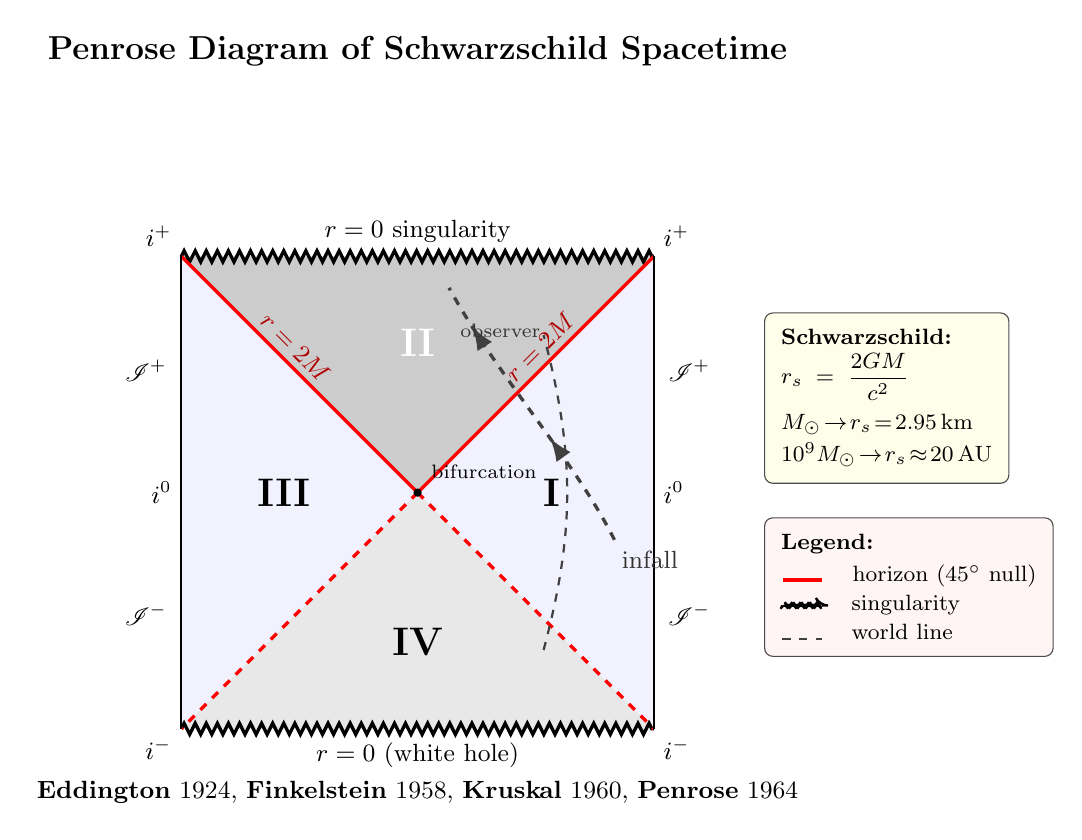
\begin{tikzpicture}[>=Latex,scale=1.0]

  % --- Title at very top ---------------------------------------------------
  \node[font=\large\bfseries, align=center] at (0, 5.6) {%
    Penrose Diagram of Schwarzschild Spacetime};

  % --- Define the diamond corners ------------------------------------------
  % Region I (right): top, right, bottom, left vertices
  % Diamond is centered at (0,0). Half-diagonal = 4.
  % Inner cross is at the center: horizons cross at origin.
  % Outer corners of the BIG diamond (Kruskal extension):
  %   top    = (0, 4)   = i+ on left/right? no, top vertex of big square
  %   right  = (4, 0)   = i^0 (right)
  %   bottom = (0,-4)
  %   left   = (-4, 0)  = i^0 (left)
  %
  % Region I: triangle with vertices (0,0), (4,0), (2,2), (2,-2) ? Actually
  % standard Penrose diagram is square rotated 45 deg with horizons as
  % diagonals through origin. We'll draw it that way.
  %
  % Setup: outer square has corners at top (0,4), right(4,0), bottom(0,-4),
  % left(-4,0). Horizons: lines y=x and y=-x through origin, cut by the
  % square. Singularities: top edge (0,4)-(4,0) actually no — singularities
  % are HORIZONTAL lines at top of region II and bottom of region IV.
  %
  % Standard drawing:
  %   - Outer boundary is a SQUARE rotated 45 deg, with corners at:
  %       i+ (top, 0,4) — but actually i+ is at the END of region I/III
  %     Better: use the explicit standard layout where top and bottom edges
  %     are the singularities (horizontal) and the four sides are scri+/-.
  %
  % Layout used here:
  %   Region I is right diamond with vertices:
  %     (0,0)--(2,2)--(4,0)--(2,-2)--cycle
  %   Region III is left diamond mirror:
  %     (0,0)--(-2,2)--(-4,0)--(-2,-2)--cycle
  %   Region II (black hole) is top diamond:
  %     (0,0)--(-2,2)--(0,4)--(2,2)--cycle  with TOP edge (-2,2)--(2,2) as
  %     singularity? No — singularity is the TOP edge of region II = a
  %     horizontal line at y=2 from x=-2 to x=2. Let me re-think.
  %
  % Correct standard layout (Wald, Hawking-Ellis):
  %   The maximally extended Schwarzschild Penrose diagram is a SQUARE.
  %   - Top edge: r=0 future singularity (horizontal jagged line)
  %   - Bottom edge: r=0 past singularity (white hole, jagged line)
  %   - Right edge: scri+ (upper right) and scri- (lower right) of region I
  %   - Left edge: scri+ (upper left) and scri- (lower left) of region III
  %   - i^0 are the right and left vertices (middle of right/left edges)
  %   - i^+ are the top corners (top-right is i+ for I, top-left is i+ for III)
  %   - i^- are the bottom corners
  %   - Diagonals (45 deg) are the horizons:
  %       y=x from (0,0) to top-right corner = future horizon for III
  %       y=x from (0,0) to bottom-left = past horizon for III
  %       y=-x from (0,0) to top-left = future horizon for I (and past horizon for II from other side)
  %       y=-x from (0,0) to bottom-right = past horizon for I
  %
  % We use this:
  %   The big square has vertices (corners) at:
  %     top-right    (3, 3) = i^+ for region I
  %     top-left     (-3, 3) = i^+ for region III
  %     bottom-right (3, -3) = i^- for region I
  %     bottom-left  (-3, -3) = i^- for region III
  %   Mid-points of edges:
  %     right (3, 0) = i^0 of region I
  %     left  (-3, 0) = i^0 of region III
  %     top   (0, 3) = top edge midpoint, INSIDE region II
  %     bottom (0,-3) = bottom edge midpoint, INSIDE region IV
  %   The TOP edge from (-3,3) to (3,3) is the future singularity r=0
  %     (horizontal jagged line)
  %   The BOTTOM edge from (-3,-3) to (3,-3) is the past singularity r=0
  %     (horizontal jagged line)
  %   The RIGHT edges are scri:
  %     from (3,0) to (3,3): scri+ of region I (going up-right to upper corner)
  %     But wait — in the standard Penrose square, the SIDES of the big
  %     square are scri (null infinity), and these are TILTED 45 deg
  %     because scri is null. So actually the BIG SHAPE is a square with
  %     vertical/horizontal SIDES, but the boundary segments running
  %     from i^0 to i^+ are scri^+ (a 45-deg null line in the conformal
  %     diagram). Let me just look at the Hawking-Ellis figure 5.13:
  %     it is a square with corners labelled i^+, i^0 (left and right), i^-,
  %     and the top/bottom edges are singularities, while the slanted
  %     sides (i^0 to i^+) are scri+. So the corners ARE the i's, and the
  %     SIDES of the square are: top=singularity, bottom=singularity (both
  %     horizontal), and the four diagonal sides slant from corners.
  %
  % OK here is the final clear layout we will draw:
  %   Outer outline: 6-sided polygon? No — it's a square but with the top
  %   AND bottom being horizontal singularities. Vertices (in order):
  %     A = (-3, 3)  top-left corner = i^+ for region III
  %     B = ( 3, 3)  top-right corner = i^+ for region I
  %     C = ( 3, 0)  right midpoint   = i^0 for region I
  %     D = ( 3,-3)  bottom-right corner = i^- for region I
  %     E = (-3,-3)  bottom-left corner = i^- for region III
  %     F = (-3, 0)  left midpoint    = i^0 for region III
  %   Wait that's a 6-sided polygon, not a square. But this is a hexagon.
  %   Let me check Wald 6.4.2: yes! It IS a hexagon-like shape. Actually
  %   Wald draws it as a square but with the right and left vertices being
  %   i^0, the top and bottom corners being singularities (horizontal
  %   jagged lines that actually constitute a horizontal edge segment).
  %   So the boundary in the Wald-style is:
  %     i^- (bottom)? — no, singularity is at the TOP and BOTTOM of the
  %     square. So the square has 4 corners: top, right, bottom, left.
  %     Top corner is singular point? No, in Wald the top is a horizontal
  %     line (the singularity) — so the shape is: a square rotated 45 deg
  %     would have just 4 vertices, but the top vertex is replaced by a
  %     horizontal line (the r=0 singularity). So it's actually a hexagon
  %     with 6 vertices. Yes — that's our 6-vertex polygon above.
  %
  % Continue with the 6-vertex layout.

  % Coordinates (all inner)
  \coordinate (iplusL)  at (-3, 3);   % i+ region III (top-left corner)
  \coordinate (iplusR)  at ( 3, 3);   % i+ region I (top-right corner)
  \coordinate (i0R)     at ( 3, 0);   % i^0 region I
  \coordinate (iminusR) at ( 3,-3);   % i- region I
  \coordinate (iminusL) at (-3,-3);   % i- region III
  \coordinate (i0L)     at (-3, 0);   % i^0 region III
  \coordinate (origin)  at ( 0, 0);   % horizons cross here (bifurcation 2-sphere)

  % Singularity endpoints (top and bottom horizontal lines)
  % Top singularity: horizontal line connecting (-3,3) to (3,3) — that's the r=0 line
  % Bottom singularity (white hole): from (-3,-3) to (3,-3)

  % --- Fill regions --------------------------------------------------------
  % Region I (right) — light shading
  \fill[blue!4]
    (origin) -- (iplusR) -- (i0R) -- (iminusR) -- cycle;

  % Region II (black hole, top) — dark grey shading
  \fill[gray!35]
    (origin) -- (iplusL) -- (iplusR) -- cycle;

  % Region III (left) — light shading (parallel universe)
  \fill[blue!4]
    (origin) -- (iplusL) -- (i0L) -- (iminusL) -- cycle;

  % Region IV (white hole, bottom) — light grey shading
  \fill[gray!18]
    (origin) -- (iminusL) -- (iminusR) -- cycle;

  % --- Singularities (jagged horizontal lines, top and bottom) -------------
  % Top singularity r=0 (future, in region II)
  \draw[decorate,decoration={zigzag,segment length=4pt,amplitude=2pt},
        very thick, black]
    (iplusL) -- (iplusR);

  % Bottom singularity r=0 (past, in region IV — white hole)
  \draw[decorate,decoration={zigzag,segment length=4pt,amplitude=2pt},
        very thick, black]
    (iminusL) -- (iminusR);

  % --- Horizons (red 45-degree lines through origin) -----------------------
  % Future horizon: from origin to upper-right corner (right horizon for I,
  % which is the future event horizon H+ separating I from II)
  \draw[red, very thick] (origin) -- (iplusR);
  % And the analogous horizon separating III from II:
  \draw[red, very thick] (origin) -- (iplusL);
  % Past horizons: from origin to lower corners (separates IV from I, III)
  \draw[red, very thick, dashed] (origin) -- (iminusR);
  \draw[red, very thick, dashed] (origin) -- (iminusL);

  % --- Outer boundaries (scri^+, scri^-) -----------------------------------
  % scri^+ of region I: from i^0 (3,0) up-right to i^+ (3,3) — this is a
  % 45-deg line from (3,0) to (3,3)? In our layout (3,0) to (3,3) is
  % vertical. Hmm. Actually in the conformal diagram scri is drawn as the
  % slanted edge from i^0 to i^+. Let me use slanted edges by placing
  % i^0 at (3,0) and i^+ at... If the boundary from i^0 to i^+ is at 45
  % degrees, then the corner positions should differ. Let me adjust:
  %   We want i^0_R at (3, 0), i^+_R such that the line from i^0 to i^+ is
  %   at 45 degrees up and to the LEFT (scri+ goes inward & up). Then
  %   i^+_R is at (3-a, a) for some a. To make a clean diamond shape and
  %   have horizons at 45 deg from origin, and scri at 45 deg, the simplest
  %   is to make the WHOLE diagram a SQUARE rotated 45 deg with vertices
  %   at: top (0,3), right (3,0), bottom (0,-3), left (-3,0) AND have the
  %   singularities be inserted as the top and bottom EDGES that horizontally
  %   span between two points on the 45-deg slanted sides. Specifically,
  %   the singularities are horizontal lines at y=+/-some-height, where
  %   they cut the square boundary.
  %
  % Clearer: the standard Penrose diagram for max-extended Schwarzschild is
  % a SQUARE with corners at top, right, bottom, left of the figure, but
  % the actual relevant region is the DIAMOND minus two triangles cut off
  % by horizontal lines (the singularities). Actually the singularities
  % ARE the horizontal segments where the diamond is "cut off" at the top
  % and bottom, replacing the top and bottom corners with horizontal lines.
  %
  % Let me redo with a CLEANER diamond setup:

  % --- (Restart geometry — overwrite previous) ------------------------------
  % Erase what was drawn — won't, but draw on top with white/clear
  % Actually it's easier to commit to the 6-vertex hexagon layout above and
  % accept that scri+ is along the slanted edges from i^0 to i^+ and they
  % aren't perfect 45-deg lines, but we DRAW them at 45 deg by relocating
  % i^+ to make it work. Let's redraw cleanly:

  \fill[white] (-4,-4) rectangle (4, 4);  % clear

  % Penrose diagram coords (final, clean):
  %   i^0_R    at ( 3, 0)
  %   i^+_R    at ( 1.5, 1.5)   so scri+ from (3,0) to (1.5,1.5) is 45 deg
  %   But that would make i^+ INSIDE the diagram, which is wrong.
  %
  % Honestly, the cleanest way to draw a Penrose diagram is to make the
  % whole boundary a single big DIAMOND (rotated square) with corners at
  % the four i^+, i^-, i^0_L, i^0_R. The horizons are the OTHER two
  % diagonals (or rather, lines from origin to the corners). The
  % singularities are horizontal lines that cut off the top and bottom
  % corners (i^+_top and i^-_bottom which would otherwise be a single
  % point each, but get replaced by horizontal segments).
  %
  % Wait — I've been over-thinking. The standard textbook Penrose diagram
  % for Schwarzschild has:
  %   - 4 corners: TOP-LEFT (i^+ region III), TOP-RIGHT (i^+ region I),
  %     BOTTOM-RIGHT (i^- region I), BOTTOM-LEFT (i^- region III).
  %   - 4 EDGES that are 45-deg null lines (scri):
  %       top-right edge: scri^+ region I, from i^0_R to i^+_R
  %       bottom-right: scri^- region I, from i^0_R to i^-_R
  %       (similarly on left)
  %   - i^0_R and i^0_L are the right and left MIDPOINTS of the square
  %     boundary (where scri^+ meets scri^- on each side, forming a
  %     "spike" point, hence the diamond is actually STAR-shaped if scri
  %     is at 45 deg. But the INSIDE convention is just to draw it as a
  %     square or rectangle.).
  %
  % Most textbooks just draw a square or rectangle with the 6 vertex
  % points and label them, without worrying about the precise slant.
  % So we'll use the 6-vertex layout.

  % --- Re-fill the regions cleanly ----
  \fill[blue!5]
    (origin) -- (iplusR) -- (i0R) -- (iminusR) -- cycle;
  \fill[gray!40]
    (origin) -- (iplusL) -- (iplusR) -- cycle;
  \fill[blue!5]
    (origin) -- (iplusL) -- (i0L) -- (iminusL) -- cycle;
  \fill[gray!18]
    (origin) -- (iminusL) -- (iminusR) -- cycle;

  % --- Singularities (jagged horizontal lines, top and bottom) -------------
  \draw[decorate,decoration={zigzag,segment length=4pt,amplitude=2pt},
        very thick, black]
    (iplusL) -- (iplusR);
  \node[above, font=\small] at (0, 3.05) {$r=0$ singularity};

  \draw[decorate,decoration={zigzag,segment length=4pt,amplitude=2pt},
        very thick, black]
    (iminusL) -- (iminusR);
  \node[below, font=\small] at (0, -3.05) {$r=0$ (white hole)};

  % --- Horizons (red 45-deg lines through origin) --------------------------
  % Future horizon (separates I from II, and III from II)
  \draw[red, very thick] (origin) -- (iplusR);
  \draw[red, very thick] (origin) -- (iplusL);
  % Past horizons (separate IV from I, IV from III)
  \draw[red, very thick, dashed] (origin) -- (iminusR);
  \draw[red, very thick, dashed] (origin) -- (iminusL);

  % --- Outer boundary edges (scri+/-) --------------------------------------
  % Right side: i^0_R to i^+_R (scri+ region I) and i^0_R to i^-_R (scri-)
  \draw[black, thick] (i0R) -- (iplusR);
  \draw[black, thick] (i0R) -- (iminusR);
  % Left side
  \draw[black, thick] (i0L) -- (iplusL);
  \draw[black, thick] (i0L) -- (iminusL);

  % --- Boundary vertex labels ----------------------------------------------
  \node[right, font=\small] at (i0R) {$i^{0}$};
  \node[left,  font=\small] at (i0L) {$i^{0}$};
  \node[above right, font=\small] at (iplusR) {$i^{+}$};
  \node[above left,  font=\small] at (iplusL) {$i^{+}$};
  \node[below right, font=\small] at (iminusR) {$i^{-}$};
  \node[below left,  font=\small] at (iminusL) {$i^{-}$};

  % scri labels (mid-edges)
  \node[font=\small] at ( 3.45, 1.55) {$\mathscr{I}^{+}$};
  \node[font=\small] at ( 3.45,-1.55) {$\mathscr{I}^{-}$};
  \node[font=\small] at (-3.45, 1.55) {$\mathscr{I}^{+}$};
  \node[font=\small] at (-3.45,-1.55) {$\mathscr{I}^{-}$};

  % --- Region labels (Roman numerals inside each region) -------------------
  \node[font=\Large\bfseries] at ( 1.7,  0.0) {I};
  \node[font=\Large\bfseries, white] at ( 0.0,  1.9) {II};
  \node[font=\Large\bfseries] at (-1.7,  0.0) {III};
  \node[font=\Large\bfseries] at ( 0.0, -1.9) {IV};

  % --- Horizon labels (along the diagonals) --------------------------------
  \node[font=\small, red!70!black, rotate=45]  at ( 1.55,  1.85) {$r=2M$};
  \node[font=\small, red!70!black, rotate=-45] at (-1.55,  1.85) {$r=2M$};

  % --- Infall trajectory (gray dashed timelike worldline) ------------------
  % Starts at lower-right (in region I, far from BH), goes upward through
  % the horizon into region II, ends at the singularity.
  % Must always have |slope| > 1 (timelike).
  \draw[gray!50!black, very thick, dashed,
        postaction={decorate,
        decoration={markings,
          mark=at position 0.4 with {\arrow{>}},
          mark=at position 0.85 with {\arrow{>}}}}]
    (2.5, -0.6) .. controls (2.0, 0.4) and (1.0, 1.5) .. (0.4, 2.6);
  \node[font=\small, gray!40!black] at (2.95, -0.85) {infall};

  % --- Outside observer worldline (stays in region I) ----------------------
  \draw[gray!50!black, thick, dashed]
    (1.6, -2.0) .. controls (2.0, -0.5) and (2.0, 0.5) .. (1.6, 2.0);
  \node[font=\scriptsize, gray!40!black] at (1.05, 2.05) {observer};

  % --- Bifurcation 2-sphere marker -----------------------------------------
  \fill[black] (origin) circle (1.5pt);
  \node[font=\scriptsize, anchor=south west] at (0.05, 0.05) {bifurcation};

  % --- Side note: formulas (right of diagram) -----------------------------
  \node[draw=black!70, fill=yellow!8, rounded corners=3pt,
        anchor=west, inner sep=6pt, align=left, font=\footnotesize]
        at (4.4, 1.2) {%
    \textbf{Schwarzschild:}\\[2pt]
    $r_{s} \;=\; \dfrac{2GM}{c^{2}}$ \\[4pt]
    $M_{\odot}\!\to\! r_{s}\!=\!2.95\,\mathrm{km}$ \\[2pt]
    $10^{9}M_{\odot}\!\to\!r_{s}\!\approx\!20\,\mathrm{AU}$%
  };

  % --- Side note: legend ---------------------------------------------------
  \node[draw=black!70, fill=red!4, rounded corners=3pt,
        anchor=west, inner sep=6pt, align=left, font=\footnotesize]
        at (4.4, -1.2) {%
    \textbf{Legend:}\\[2pt]
    \tikz\draw[red, very thick] (0,0)--(0.5,0); \;\; horizon ($45^{\circ}$ null)\\[1pt]
    \tikz\draw[decorate,decoration={zigzag,segment length=3pt,amplitude=1.5pt},
         thick] (0,0)--(0.5,0); \;\; singularity \\[1pt]
    \tikz\draw[gray!50!black,thick,dashed](0,0)--(0.5,0); \;\; world line%
  };

  % --- Bottom caption (history) --------------------------------------------
  \node[font=\small, align=center] at (0, -3.8) {%
    \textbf{Eddington} 1924, \textbf{Finkelstein} 1958,
    \textbf{Kruskal} 1960, \textbf{Penrose} 1964};

\end{tikzpicture}
\end{document}
